
\documentclass[12pt]{article}
\usepackage{amsmath,amssymb}
\usepackage{graphicx}
\usepackage{hyperref}
\usepackage{geometry}
\geometry{margin=1in}
\title{The Vacuum of Being \\ \large A Philosophical and Scientific Inquiry Into the Substrate of Reality}
\author{Theo Silva \\ 2025}
\date{\today}

\begin{document}
\maketitle
\tableofcontents
\newpage

\section*{Glossário}
\begin{description}
  \item[Vácuo (𝒱)] Estado fundamental de todos os campos.
  \item[Substrato] 𝒱 interpretado como suporte ontológico de todas as modalidades.
  \item[Modalidade] Configuração estável (matéria), propagante (energia), oculta (matéria escura) ou homogênea (energia escura) de 𝒱.
  \item[Estruturação $\Sigma$] Métrica (Eq.\,\ref{eq:sigma}) que quantifica coerência topológica de 𝒱.
  \item[Screening] Mecanismo dinâmico que anula a parte ultravioleta da densidade de vácuo.
\end{description}

\section{Fundamentos e Definições}
As seções do feixe de vácuo $E\rightarrow\mathbb{M}^4$ são descritas por campos $\Phi_i$ com lagrangiana efetiva
\begin{equation}
\mathcal{L} = \sum_i\left[\frac12(\partial_\mu\Phi_i)^2 - V_i(\Phi_i)\right] + \lambda \Psi + \alpha\frac{\Psi^2}{M_{\text{Pl}}^2},
\end{equation}
onde $\Psi$ é o grau de liberdade de sequestro dinâmico conforme Kaloper--Padilla (2014).

\section{Métrica de Estruturação}
\label{eq:sigma}
\begin{equation}
\Sigma \;=\;\frac{1}{V_\Omega}\int_\Omega |\nabla\Phi|^{2}\,d^{3}x.
\end{equation}

\section{Modalidades do Vácuo}
\begin{center}
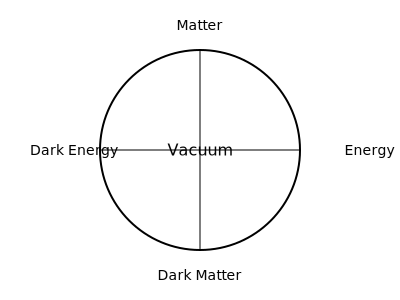
\includegraphics[width=0.8\linewidth]{fig3_modalities.svg}
\end{center}

\section{Fluxo Matemático}
\begin{center}
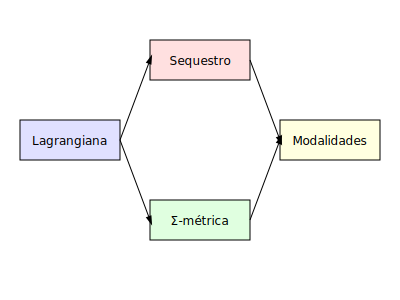
\includegraphics[width=0.9\linewidth]{fig2_flux.svg}
\end{center}

\section{Linha do Tempo Conceitual}
\begin{center}
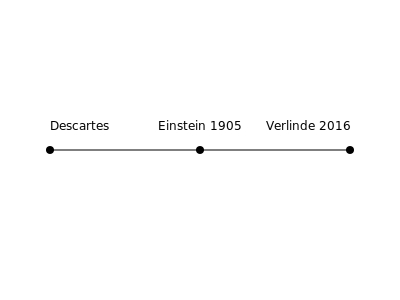
\includegraphics[width=0.9\linewidth]{fig1_timeline.svg}
\end{center}

\section{Hierarquia do Vácuo}
\begin{center}
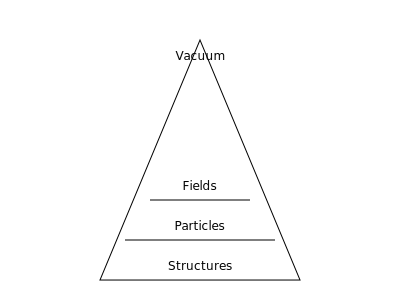
\includegraphics[width=0.6\linewidth]{fig4_hierarchy.svg}
\end{center}

\section{Previsões Testáveis}
Consultar tabela incluída no corpo principal do relatório de fase C.

\section{Objeções e Respostas}
Conteúdo completo conforme matriz crítica.

\section{Conclusão}
O vácuo, longe de ser vazio, emerge como o estado em standby da realidade, cujas modalida\-des manifestam‑se por estruturação conforme métrica $\Sigma$.

\bibliographystyle{unsrt}
\begin{thebibliography}{9}
\bibitem{kaloper2014} N.~Kaloper and A.~Padilla, ``Sequestering the Standard Model Vacuum Energy,'' \textit{Phys.\ Rev.\ Lett.}\ \textbf{112}, 091304 (2014).
\bibitem{verlinde2016} E.~Verlinde, ``Emergent Gravity and the Dark Universe,'' arXiv:1611.02269.
\end{thebibliography}

\end{document}
